% !TEX TS-program = xelatex
\documentclass[11pt]{article}
\usepackage{xcolor}
\usepackage{lindrew}
\usepackage{tikz}
\usepackage{pgfplots}
\usepackage{fontspec}
\pgfplotsset{compat=1.18}
\title{Math 4580: Abstract Algebra I}
\author{Lecturer: \textbf{Professor Michael Lipnowski}\\Notes by: Farhan Sadeek}
\date{Spring 2025}

\begin{document}

\maketitle
%%%%%%%%%%%%%%%%%%%%%%%%%%%%

\section{January 6, 2025}
We didn't have any, but Dr.\ Lipnowski did post a module on
\href{https://carmen.osu.edu}{\texttt{carmen}} about the syllabus and the
course. This semester we will be covering the first few chapters of the book
\textit{Abstract Algebra: Theory and Applications} by Thomas Judson. \\

\begin{definition}
    \vocab{Set}: A collection of distinct objects, considered as an object in its own right.\\
    \vocab{Axioms}: A collection of objects \( \mathrm{S} \) with assumed structural rules is defined by axioms.\\
    \vocab{Statement}: In logic or mathematics, an assertion that is either true or false.\\
    \vocab{Hypothesis and Conclusion}: In the statement ``If P, then Q'', P is the hypothesis and Q is the conclusion.\\
    \vocab{Mathematical Proof}: A logical argument that verifies the truth of a statement.\\
    \vocab{Proposition}: A statement that can be proven true.\\
    \vocab{Theorem}: A proposition of significant importance.\\
    \vocab{Lemma}: A supporting proposition used to prove a theorem or another proposition.\\
    \vocab{Corollary}: A proposition that follows directly from a theorem or proposition with minimal additional proof.
\end{definition}

\section{January 8, 2025}
Professor Lipnowski discussed Sam Lloyd's 15 puzzle. Each lecture will include
a mystery digit, contributing up to 5\% bonus to the final grade based on
correct guesses.

Certain course expectations:
\begin{itemize}
    \item All assignments (one every two weeks) and exams (one midterm and one final
          exam) will be take-home.
    \item All the problems from the course textbook.
    \item Collaboration is encouraged, but the work should be your own.
    \item For the exams, we are not supposed to talk to other friends.
\end{itemize}

\subsection{Functions}
\begin{definition}
    Let $A$ and $B$ be sets. A function $f: A \to B$ assigns exactly one output $f(a) \in B$ to every input $a \in A$.
\end{definition}
\begin{itemize}
    \item The set $A$ is called the \textbf{domain} of $f$.
    \item The set $B$ is called the \textbf{codomain} of $f$.
\end{itemize}

\begin{fact}The domain $A$, codomain $B$, and the assignment of outputs $f(a)$ to every input $a \in A$ are all part of the data defining a function. Just writing a formula like $f(x) = e^x$ does not determine a function, as the domain and codomain are not specified. 
\end{fact}
For example:
\begin{itemize}
    \item $f: \mathbb{R} \to \mathbb{R}, f(x) = e^x$.
    \item $f: \mathbb{Q} \to \mathbb{Q}, f(x) = e^x$.
\end{itemize}
Although these functions use the same formula, their meanings are completely different because their domains and codomains differ.

\subsection{Graphs}
A function $f: A \to B$ is often identified with its \textbf{graph} in $A
    \times B$:
\[ \text{graph}(f) = \{(a, b) \in A \times B : b = f(a)\}. \]

\begin{lemma}
    Let $f: A \to B$ be a function. Its graph, $\text{graph}(f)$, passes the \textbf{vertical line test}: For every $a \in A$, $V_a := \{(a, b) \in A \times B : b \in B\}$ intersects $\text{graph}(f)$ in exactly one element.
\end{lemma}
\begin{center}
    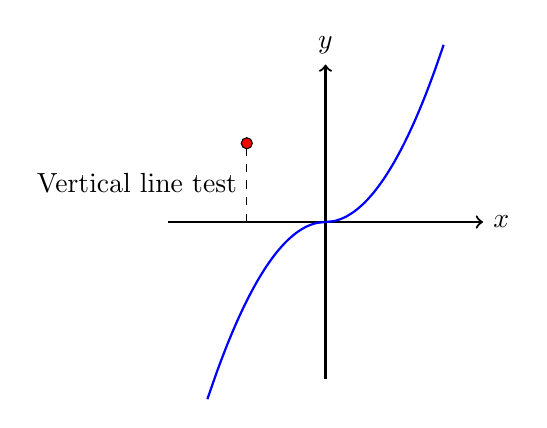
\begin{tikzpicture}
        \draw[thick,->] (-2,0) -- (2,0) node[right] {$x$};
        \draw[thick,->] (0,-2) -- (0,2) node[above] {$y$};
        \draw[domain=-1.5:1.5,smooth,variable=\x,blue,thick] plot ({\x},{\x^2});
        \draw[dashed] (-1,0) -- (-1,1) node[midway,left] {Vertical line test};
        \draw[fill=red] (-1,1) circle (2pt);
    \end{tikzpicture}
\end{center}

\begin{proposition}
    Let $G \subseteq A \times B$ be any subset passing the vertical line test, i.e., for all $a \in A$, $V_a \cap G$ consists of exactly one element. Then $G = \text{graph}(f)$ for a unique function $f: A \to B$.
\end{proposition}
\begin{proof}
    If $G = \{(a, b) \mid b \in B\}$ satisfies the vertical line test, define $f: A \to B$ by $f(a) = b$. Then $G = \text{graph}(f)$.
\end{proof}

\begin{definition}
    A subset $R \subseteq A \times B$ is called a \textbf{relation}. The vertical line test distinguishes graphs of functions from more general relations.
\end{definition}
\section*{Examples}
\begin{itemize}
    \item Let $S = \{(x, y) \in \mathbb{R}^2 : x^2 + y^2 = 1\}$ (the unit circle). This
          is a relation but not the graph of a function because it fails the vertical
          line test: The vertical line $x = 0$ intersects the circle at two points.
    \item Visual depiction of a unit circle:
          \begin{center}
              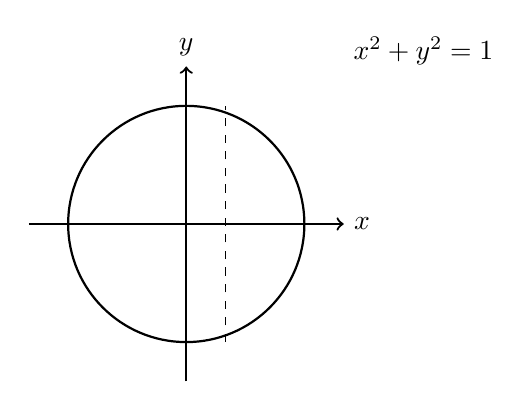
\begin{tikzpicture}
                  \draw[thick,->] (-2,0) -- (2,0) node[right] {$x$};
                  \draw[thick,->] (0,-2) -- (0,2) node[above] {$y$};
                  \draw[thick] (0,0) circle (1.5);
                  \node[below right] at (2,2.5) {$x^2 + y^2 = 1$};
                  \draw[dashed] (0.5,-1.5) -- (0.5,1.5);
              \end{tikzpicture}
          \end{center}
    \item Let $A = \{1, 2, 3\}$, $B = \{4, 5\}$. The number of functions from $A$ to $B$
          is $2^3 = 8$, corresponding to the $8$ associated graphs in $A \times B$.
    \item The number of relations from $A$ to $B$ is $2^{|A| \cdot |B|} = 2^{3 \cdot 2} =
              64$, containing the $8$ graphs of functions from $A$ to $B$.
\end{itemize}

\begin{fact}
    The notion of relation is much more permissive than the notion of functions.
\end{fact}

\section*{Visualizing Functions as Directed Edges}
A function $f: A \to B$ can be visualized as a collection of directed edges $(a, f(a)) \in A \times B$. Each element of $A$ has exactly one outgoing edge in the graph.

\begin{center}
    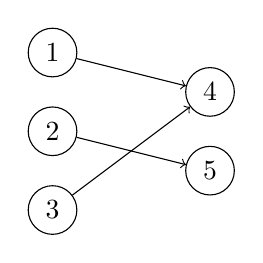
\begin{tikzpicture}
        \node[circle,draw] (A1) at (0,1) {$1$};
        \node[circle,draw] (A2) at (0,0) {$2$};
        \node[circle,draw] (A3) at (0,-1) {$3$};
        \node[circle,draw] (B1) at (2,0.5) {$4$};
        \node[circle,draw] (B2) at (2,-0.5) {$5$};
        \draw[->] (A1) -- (B1);
        \draw[->] (A2) -- (B2);
        \draw[->] (A3) -- (B1);
    \end{tikzpicture}
\end{center}

%\section{January 15, 2025}
%\section{January 17, 2025}
%\section{January 20, 2025}
%\section{January 22, 2025}
%\section{January 24, 2025}
%\section{January 27, 2025}
%\section{January 29, 2025}
%\section{January 31, 2025}
%\section{February 3, 2025}
%\section{February 5, 2025}
%\section{February 7, 2025}
%\section{February 10, 2025}
%\section{February 12, 2025}
%\section{February 14, 2025}
%\section{February 17, 2025}
%\section{February 19, 2025}
%\section{February 21, 2025}
%\section{February 24, 2025}
%\section{February 26, 2025}
%\section{February 28, 2025}
%\section{March 3, 2025}
%\section{March 5, 2025}
%\section{March 7, 2025}
%\section{March 17, 2025}
%\section{March 19, 2025}
%\section{March 21, 2025}
%\section{March 24, 2025}
%\section{March 26, 2025}
%\section{March 28, 2025}
%\section{March 31, 2025}
%\section{April 2, 2025}
%\section{April 4, 2025}
%\section{April 7, 2025}
%\section{April 9, 2025}
%\section{April 11, 2025}
%\section{April 14, 2025}
%\section{April 16, 2025}
%\section{April 18, 2025}
%\section{April 21, 2025}
%\section{April 23, 2025}
%\section{April 25, 2025}
%\section{April 28, 2025}

\end{document}
